Тестирование  на парах модельных изображений и на изображениях поверхностях реальных образцов.
\subsection{Образцы изображений}
\subsubsection{Модельные изображения}\label{mod_image}

Модельное изображение (рисунок~\ref{pic:gray_mix}) получали из заданного количества слоёв псевдослучайных чисел; при этом каждый слой соответствует определённой пространственной частоте~\cite{pan_15}. 

Первый слой некоторого заданного исходного размера заполняется псевдослучайными значениями с равномерным распределением. Затем размер данного слоя увеличивается в два раза с помощью интерполирования бикубическим Б-сплайном. Второй слой формируется аналогично первому, но перед увеличением его размера он складывается попиксельно с первым. 
Итеративно генерируются несколько слоёв, и на каждой итерации конечный размер изображения увеличивается в два раза. После генерации всех слоёв, проводится масштабирование и нормировка яркости в диапазоне от 0 до 255. Таким образом, имея начальный слой размером $4 \times 4$ пиксела, после проведения 8 итераций, получаем модельное изображение размером $1024 \times 1024$ пикселов.

Модель спекла (окрашенной поверхности). При создании модельного изображения спекла (рисунок~\ref{pic:gray_mix}) (вторая серия) стояла задача создания изображения подобного экспериментально получаемым при фотографировании образца (рисунок~\ref{pic:al_deform}). Для этого изображение ``заливали'' цветом, подобным по тону оттенку поверхности образца на экспериментально регистрируемых фотографиях. 

Затем в ``случайно'' заданных (по нормальному закону распределения) участках генерировали окружности (имитирующие капли распыляемой краски – пятна спекла), радиусом (0 до 10 пикселов), уровень (градация) серого которых задавался случайным образом. Описание изображений находится в таблице~\ref{tab:set_image}, текстуры изображены на рисунке~\ref{pic:gray_mix}.

\begin{figure}[h!]
\center{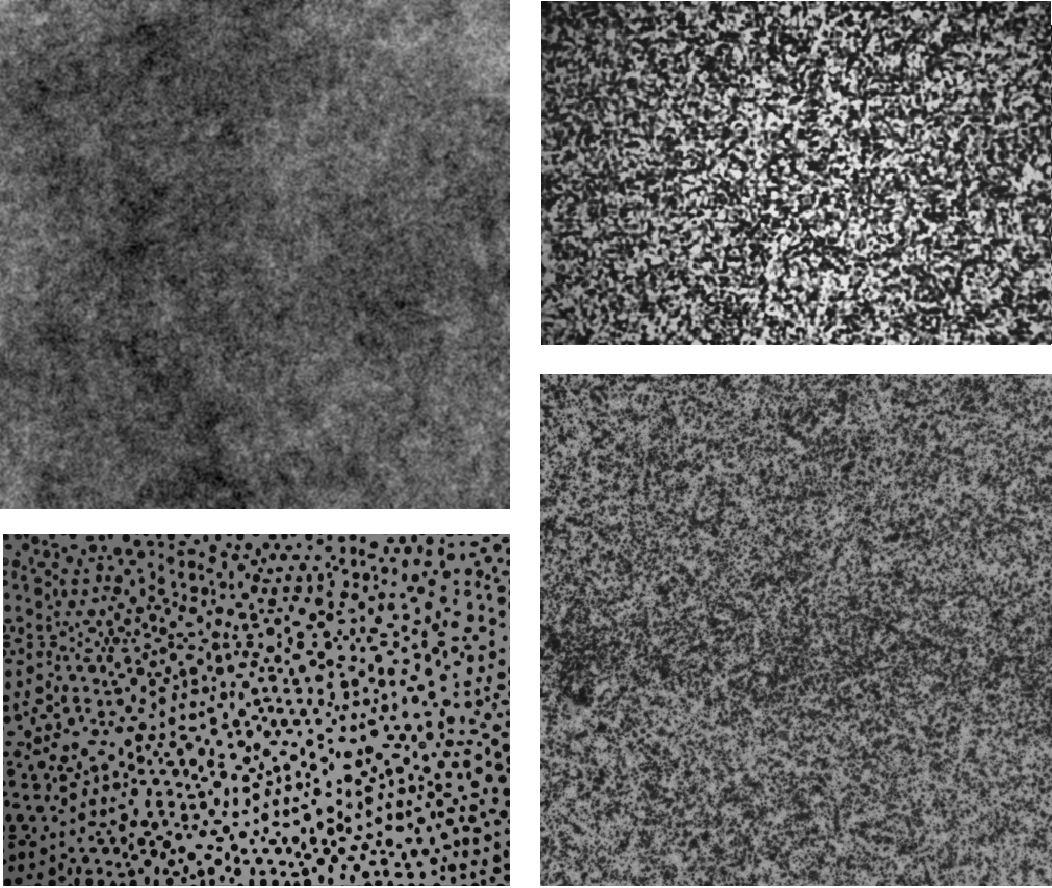
\includegraphics[width=0.9\linewidth]{gray_mix}}
\caption{Серия изображений: а) Модель многослойного изображения, б) Модель спекла}
\label{pic:gray_mix}
\end{figure}

\begin{longtable}[h!]{|m{0.4\textwidth}|m{0.12\textwidth}|m{0.11\textwidth}|m{0.08\textwidth}|m{0.15\textwidth}|}
\caption{Сравнение тестовых изображений}
\label{tab:set_image}
\\ \hline
Серия & Диапазон яркостей 	& Уровень шума & Сдвиг (px) &  Размеры \\ \hline
Модель многослойного изображения & 0-188 & Нет & 1-20 &  510$\times$510 \\ \hline
Модель спекла & 0-188 & Нет & 1-70 &  512$\times$512 \\ \hline
Пластина алюминия Д16АТ & 13-228 & Неизв. & 1-20 &  1920$\times$1080\\ \hline
\end{longtable}
\subsubsection{Реальные отснятые изображения}

Реально отснятые изображения предоставлены сотрудником ИФПМ СО РАН. 
\begin{figure}[ht!]
\center{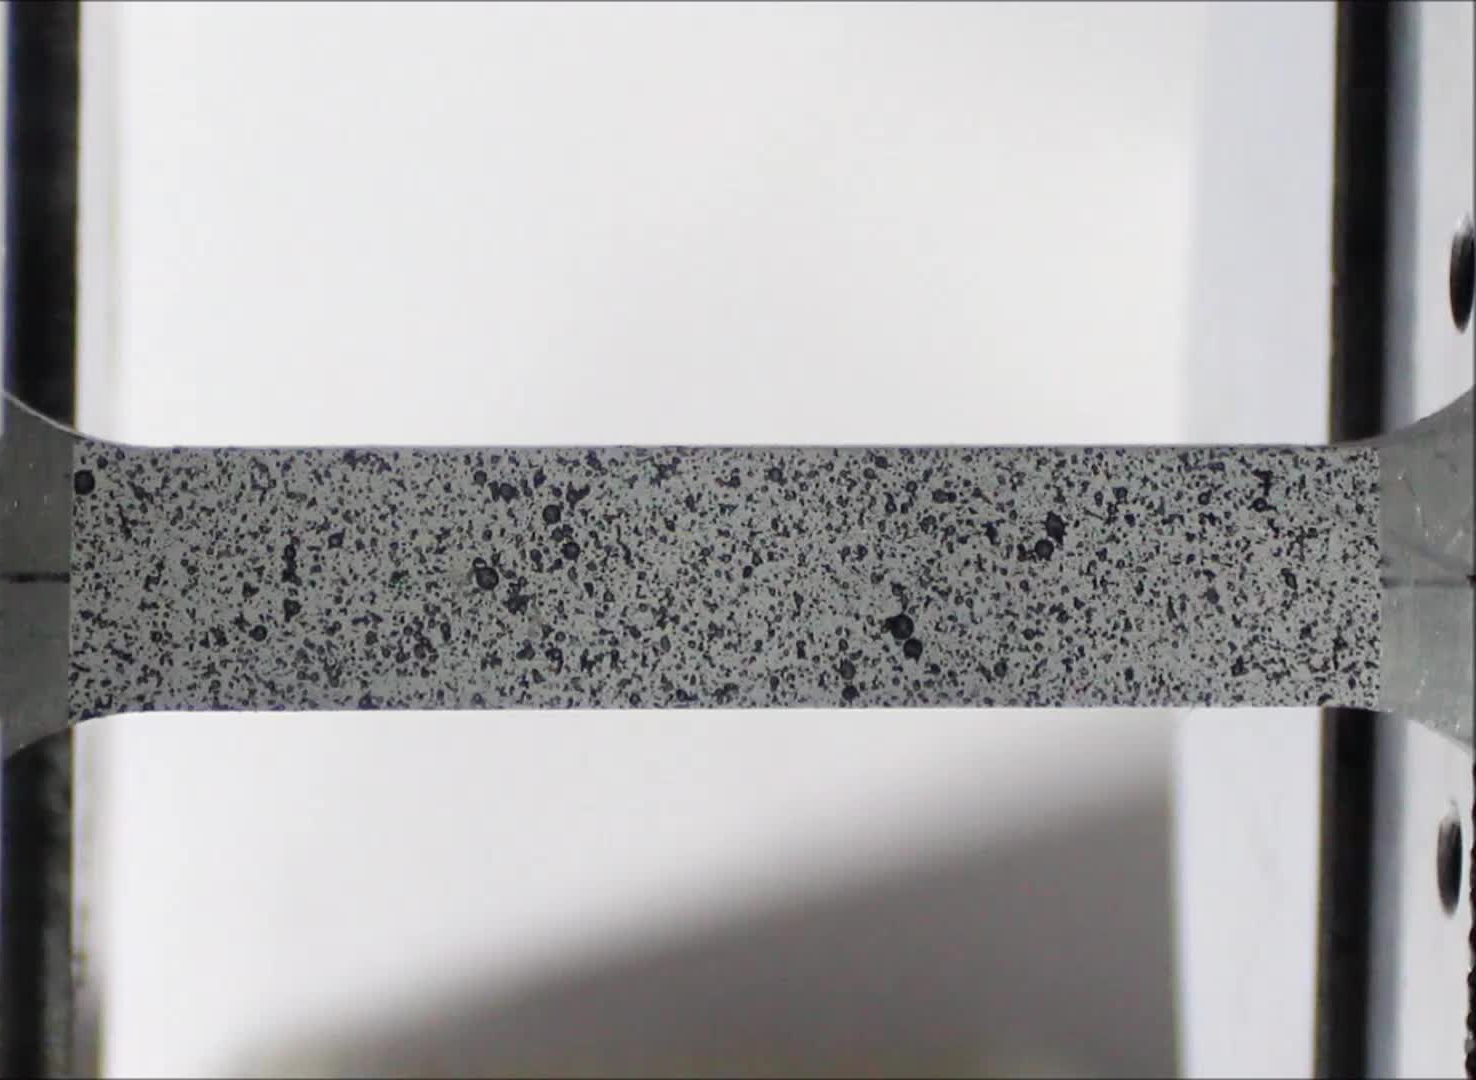
\includegraphics[width=0.6\linewidth]{al_deform}}
\caption{Растяжение пластины алюминия Д16АТ}
\label{pic:al_deform}
\end{figure}
На первой серии (рисунок~\ref{pic:al_deform}) изображён металлический образец из авиационного алюминиевого сплава Д16АТ нагружавшиеся на механической испытательной машине ИМАШ-2078 в условиях одноосного статического растяжения. Схема эксперимента на рисунке~\ref{fig:gap_mach}.
\begin{figure}[ht!]
\centering
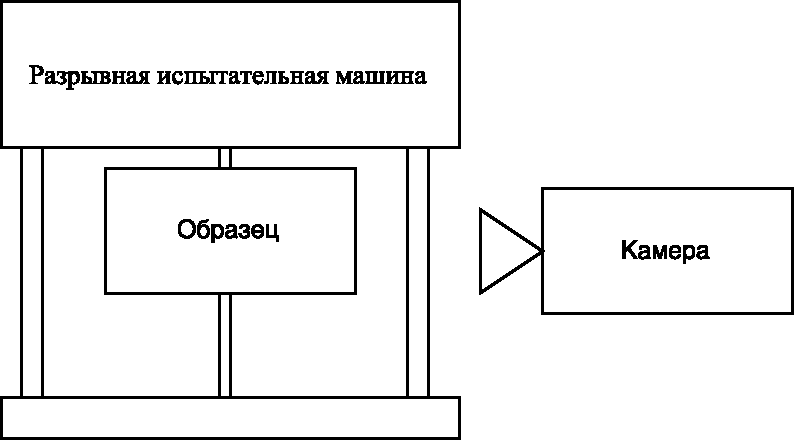
\includegraphics[width=0.7\linewidth]{images/gap_mach-crop.pdf}
\caption{Схема эксперимента}
\label{fig:gap_mach}
\end{figure}
%Размеры предоставленных изображений $1920\times1280$ пикселей.
\subsection {Оценка быстродействия}
Для проведения расчётов использовали ПЭВМ со следующими характеристиками:

Аппаратная составляющая:
\begin{itemize}
\item процессор Intel(R) Core(TM) i3 370M @ 2,4 ГГц, 64-бит;
\item оперативная память 4 Гб, 1067 МГц;
\item материнская плата Aspire 573
\item жёсткий диск SSD Smartbuy 120 Гб;
\item файловая система ext4, 107 Гб.
\end{itemize}
Программная составляющая:
\begin{itemize}
\item операционная система Linux Mint 3.19-18;
\item версия cmake 3.2.1;
\item версия QMake 3.0 \& Qt version 5.2.1;
\item версия компилятора gcc (Ubuntu 4.8.2-19ubuntu1) 4.8.2;
\item оболочка для среды рабочего стола Cinnamon 2.4.8.
\end{itemize}

Для исследования быстродействия и помехоустойчивости алгоритмов были использованы описанные ранее серии изображений.
\subsection{Тестирование программного обеспечения}
\subsubsection{Тестирование на модельных изображениях}
%Результатом работы ПО, как описано в * разделе, является векторное поле и поля деформации твёрдого тела представленное на рисунке~\ref{pic:gray_set_out}.

Программное обеспечение будет тестироваться по модели белого ящика. Входные данные для тестирования описаны в разделе~\ref{mod_image}, алгоритм работы описан на рисунке~\ref{pic:shema_PO}.

Для оценки выходных данных, мы используем модельное изображение (рисунок~\ref{pic:gray_mix} а), и сдвинем исходный рисунок по оси $x$ на один пиксель влево, по $y$ сдвиг отсутствует.
В таком случае, программа должна вычислить вектороек поле перемещений, оценить общий сдвиг, а после вычислить компоненты деформации. Так как сдвиг по всему изображению равномерный то и деформация, в этом случае отсутствует. В идеальных условиях программа должна вернуть нулевое поле (поле, заполненное нулями), однако любое измерение сопровождается некой ошибкой, все значения отличные от нуля, будут считаться ошибкой.

\subsubsection{Тестирование на экспериментально полученных изображения}
Результаты тестирования разрабатываемого программного обеспечения на изображениях поверхностей реальных образцов представлены на рисунке~\ref{fig:al_strain}.

\begin{figure}
\centering
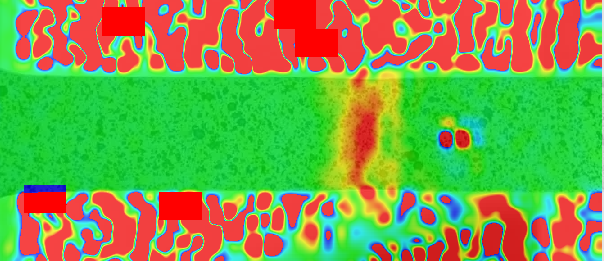
\includegraphics[width=0.7\linewidth]{images/al_strain}
\caption{Результат работы программы: нижний слой -- исходное изображение, верхний слой -- поле деформации по оси $x$ с 30\% альфа каналом}
\label{fig:al_strain}
\end{figure}
Оценить данный эксперимент не представляется возможным, так как отсутствуют данные о истинных значениях поверхностной деформации, и о цифровом  шуме фотосенсора, который использовались, для получения изображения.

\subsection{Исследование метода интерполяции}
В работе рассматривались два метода интерполяции:
\begin{itemize}
\item билинейная;
\item в-сплайн.
\end{itemize}
Как сказано ранее, все существующие методы направлены либо на улучшение быстродействия, либо на шумоустойчивость. 
\begin{figure}
\centering
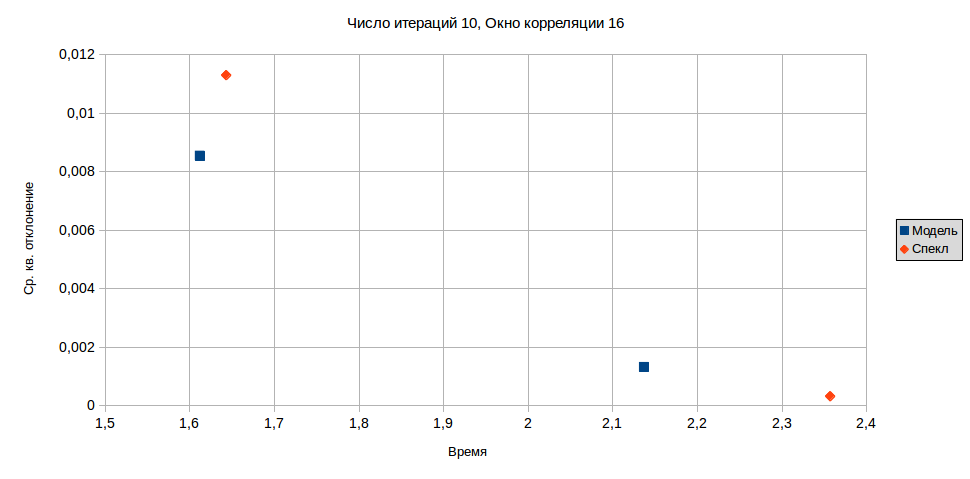
\includegraphics[width=0.8\linewidth]{images/srav_iterpol.png}
\caption{Сравнение методов интерполяции}
\label{fig:srav_iterpol}
\end{figure}
Соответственно, сравнятся будет уровень ошибки для разных реализаций, и время работы (рисунок~\ref{fig:srav_iterpol}).

Билинейный имеет наилучшее быстродействие (меньшее время работы), за счёт упрощённой математики, но не так точен, как В-сплайн. В среднем реализация билинейной интерполяции быстрее в-сплайна на ~30\%, но проигрыш в точности в 10 раз. Исходя из этого, решено использовать для остальных тестирований в-сплайновую интерполяцию. 
\subsection{Исследование числа итераций}

Реализация итеративного алгоритма значительно увеличивает точность работы программы~(рисунок~\ref{pic:inter_err}), а так же даёт возможность нахождения перемещений до 20 пикселей. С другой стороны, увеличение числа итераций ведёт к снижению быстродействия~(рисунок~\ref{pic:iter_time}).
\begin{figure}[h!]
\center{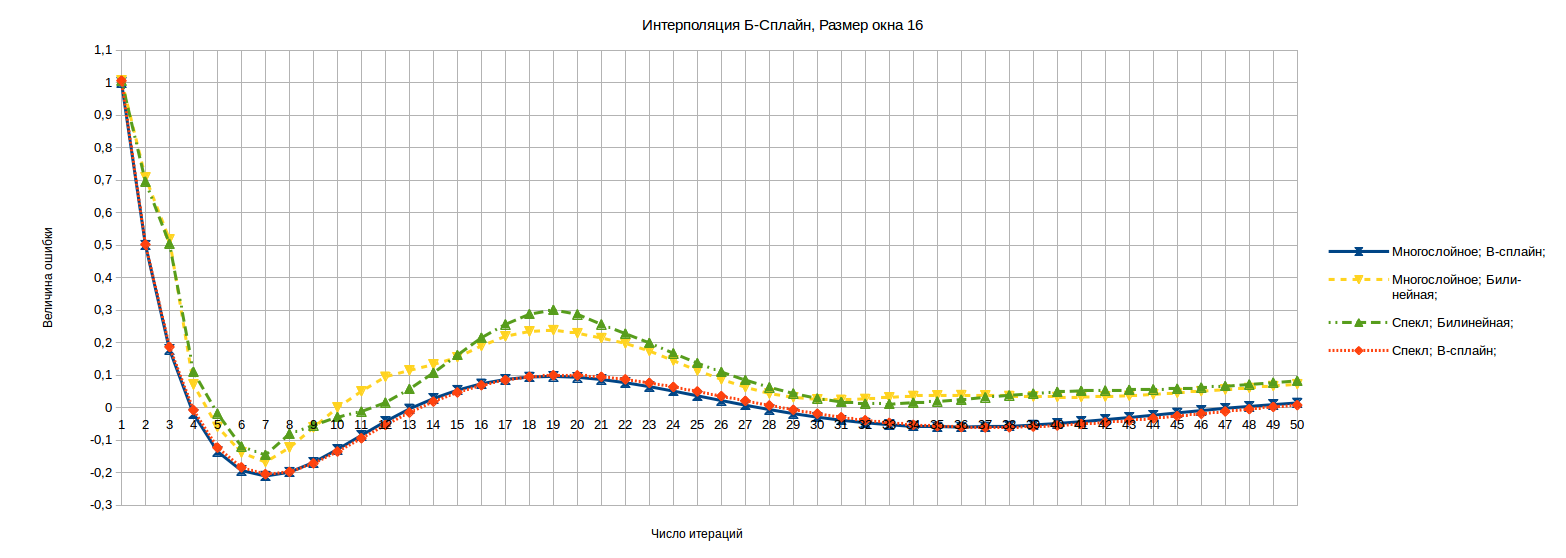
\includegraphics[width=0.9\linewidth]{images/inter_err.png}}
\caption{Величина ошибки от числа итераций}
\label{pic:inter_err}
\end{figure}

\begin{figure}[h!]
\center{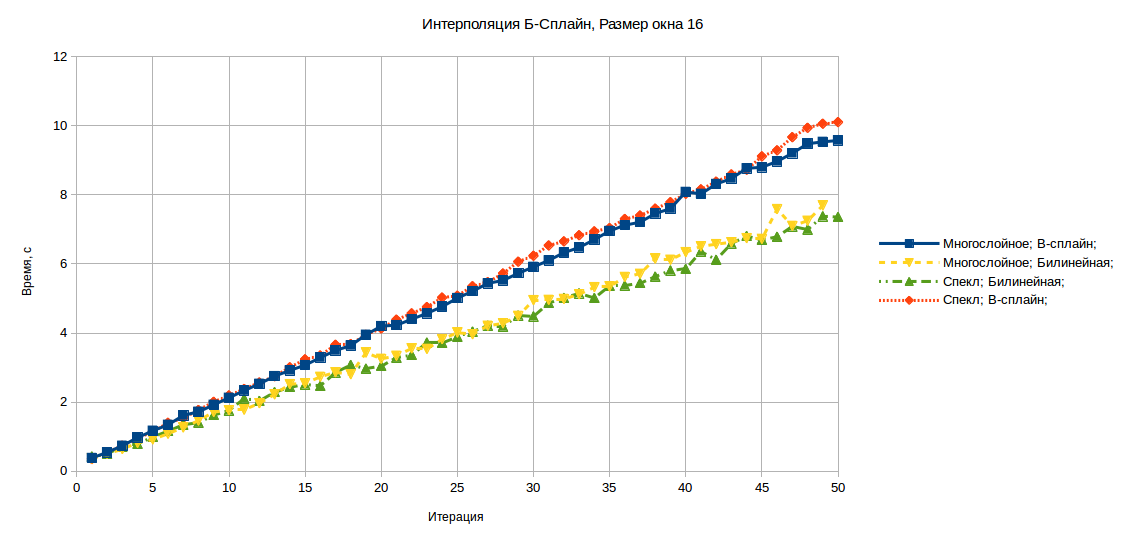
\includegraphics[width=0.9\linewidth]{images/iter_time.png}}
\caption{Время работы программы, в зависимости от числа итераций}
\label{pic:iter_time}
\end{figure}
\subsection{Исследование размера области поиска}

Увеличение области поиска положительно сказывается на работе программы (рисунок~\ref{fig:window_error}), так же нужно помнить, что реализованный алгоритм -- локален и не может вычислить сдвиг больший чем заданное окно. Однако с увеличением размера окна, возрастёт число вычислений, соответственно время работы программы увеличивается, это зависимость представлена на рисунке~\ref{pic:window_time}.
\begin{figure}
\centering
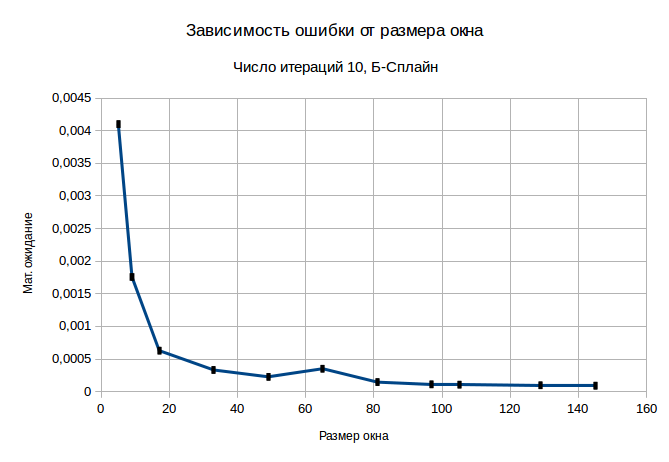
\includegraphics[width=0.9\linewidth]{images/window_error}
\caption{Величина ошибки в зависимости от размера области поиска}
\label{fig:window_error}
\end{figure}

\begin{figure}[h!]
\center{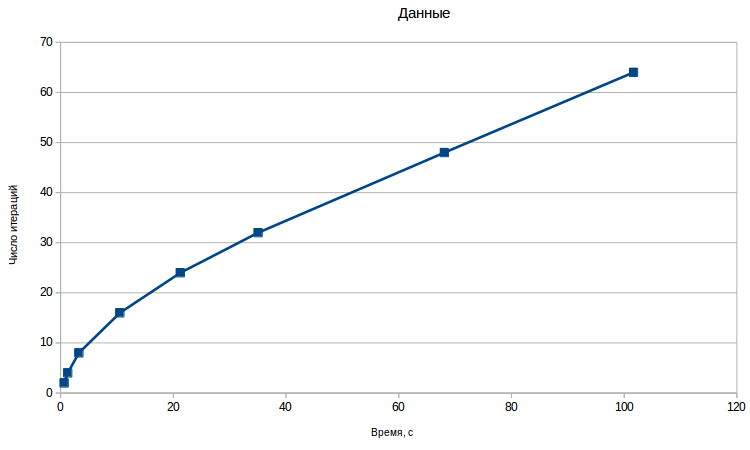
\includegraphics[width=0.9\linewidth]{images/window_time.png}}
\caption{Время работы программы, в зависимости от размера области поиска}
\label{pic:window_time}
\end{figure}
